\documentclass[a4paper,10pt]{article}
\usepackage[utf8]{inputenc}
\usepackage{tikz}
\usepackage{amsmath}
\usepackage{hyperref}
\usepackage{subcaption}
\usetikzlibrary{decorations.pathmorphing,patterns}
\usetikzlibrary{calc,patterns,decorations.markings}
\usetikzlibrary{positioning}
\usetikzlibrary{quotes,angles}

\hypersetup{
	colorlinks,
	citecolor=black,
	filecolor=black,
	linkcolor=red,
	urlcolor=red,
}

%opening
\title{The Coupled Pendulum}
\author{Jay Khandkar}

\begin{document}

\date{}
\maketitle

\section{Two Coupled Pendulums}

\begin{figure}[!h]
\centering
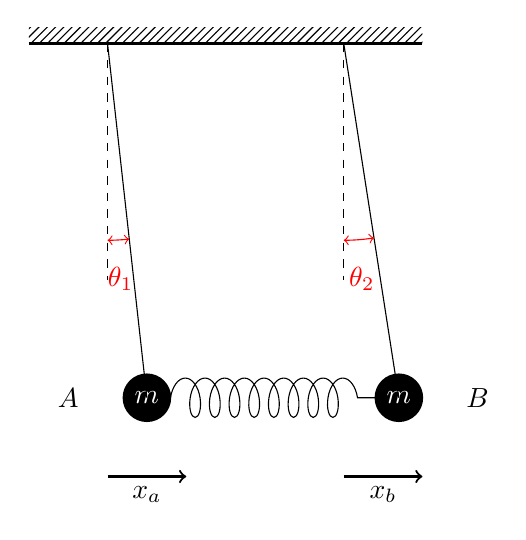
\begin{tikzpicture}
\coordinate (a) at ($(0,0)+(0.5,0.5)$);
\coordinate (b) at ($(3,0)+(0.7,0.5)$);
\coordinate (pivot1) at (0,5);
\coordinate (pivot2) at (3,5);
\node[circle,fill=black,inner sep=1mm] at (a) {$\textcolor{white}{m}$};
\node[circle,fill=black,inner sep=1mm] at (b) {$\textcolor{white}{m}$};
\node at ($(a)+(-1,0)$) {$A$};
\node at ($(b)+(1,0)$) {$B$};
\draw[decoration={aspect=0.5, segment length=2.5mm, amplitude=2.5mm,coil},decorate] ($(a)+(0.3,0)$) -- ($(b)+(-0.3,0)$); 
\draw (pivot1) -- (a); 
\draw (pivot2) -- (b); 
\draw[dashed] (0,5) -- ++(0,-3) node (end1){};
\draw[dashed] (3,5) -- ++(0,-3) node (end2){};
\draw [->, thick] ($(0,5)+(0,-5.5)$) -- ++(1,0);
\node[anchor=north] at ($(0,5)+(0.5,-5.5)$) {$x_a$};
\draw [->, thick] ($(3,5)+(0,-5.5)$) -- ++(1,0);
\node[anchor=north] at ($(3,5)+(0.5,-5.5)$) {$x_b$};
\draw pic["$\textcolor{red}{\theta_1}$",draw=red,<->,angle eccentricity=1.2, angle radius=2.5cm] {angle=end1--pivot1--a};
\draw pic["$\textcolor{red}{\theta_2}$",draw=red,<->,angle eccentricity=1.2, angle radius=2.5cm] {angle=end2--pivot2--b};
\fill [pattern = north east lines] (-1,5) rectangle (4,5.2);
\draw[thick] (-1,5) -- (4,5);
\end{tikzpicture}
\caption{Two pendulums coupled by an ideal spring}
\label{figure:two_cp_pendulums}
\end{figure}

Consider two pendulums of equal mass $m$, $A$ and $B$, coupled by an ideal massless spring of spring constant $k$, as shown in Figure \ref{figure:two_cp_pendulums}.
The string may be considered sufficiently light so that it's mass may be neglected compared to the bobs.
The equations of motion, considering small angle approximations ($\sin{\theta} \approx \theta, \ddot y \approx 0$), for the two pendulums are

\begin{align*}
m\frac{d^2x_a}{dt^2} &= -mg\frac{x_a}{l} + k(x_b - x_a)\\
m\frac{d^2x_b}{dt^2} &= -mg\frac{x_b}{l} - k(x_b - x_a)
\end{align*}
or

\begin{align}
\label{equation:two_cp_pendulums_1}
\ddot x_a + (\omega_0^{2} + \omega_c^{2})x_a - \omega_c^{2}x_b= 0\\
\label{equation:two_cp_pendulums_2}
\ddot x_b + (\omega_0^{2} + \omega_c^{2})x_b - \omega_c^{2}x_a= 0
\end{align}

where we have let $\omega_0^2 = \frac{g}{l}$ and  $\omega_c^2 = \frac{k}{m}$

\section{Normal Modes}

Before we try to solve equations \ref{equation:two_cp_pendulums_1} and \ref{equation:two_cp_pendulums_2} for the most general motion of the system,
let us consider what happens when we draw both $A$ and $B$ aside by equal amounts and release them. The spring remains relaxed and exerts no force
on either masses. Both of them then oscillate with the same natural frequency $\omega_0$:

\begin{align*}
x_a &= C\cos{\omega_0t}\\
x_b &= C\cos{\omega_0t}
\end{align*}

This is known as a \textit{normal mode of oscillation}, where all masses oscillate with the same frequency. For this system, there is yet another
normal mode: pull $A$ and $B$ aside by equal amounts but in opposite direction. The equation of motion for $A$ is 

\begin{align*}
\ddot x_a + (\omega_0^{2} + 2\omega_c^{2})x_a = 0\\
\end{align*}

which is readily identified as a simple harmonic motion of frequency $\omega\prime = (\omega_0^2 + 2\omega_c^2)^{1/2}$, so that

\begin{align*}
x_a &= C\cos{\omega^{'}t}\\
x_b &= -C\cos{\omega^{'}t}
\end{align*}

The two normal modes are illustrated in figure \ref{fig:cp_two_normal}.

\begin{figure}[!h]
\centering
\begin{subfigure}{.5\textwidth}
\centering

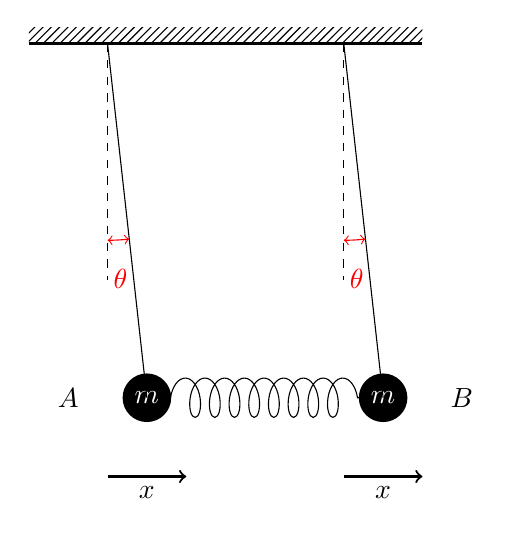
\begin{tikzpicture}
\coordinate (a) at ($(0,0)+(0.5,0.5)$);
\coordinate (b) at ($(3,0)+(0.5,0.5)$);
\coordinate (pivot1) at (0,5);
\coordinate (pivot2) at (3,5);
\node[circle,fill=black,inner sep=1mm] at (a) {$\textcolor{white}{m}$};
\node[circle,fill=black,inner sep=1mm] at (b) {$\textcolor{white}{m}$};
\node at ($(a)+(-1,0)$) {$A$};
\node at ($(b)+(1,0)$) {$B$};
\draw[decoration={aspect=0.5, segment length=2.5mm, amplitude=2.5mm,coil},decorate] ($(a)+(0.3,0)$) -- ($(b)+(-0.3,0)$); 
\draw (pivot1) -- (a); 
\draw (pivot2) -- (b); 
\draw[dashed] (0,5) -- ++(0,-3) node (end1){};
\draw[dashed] (3,5) -- ++(0,-3) node (end2){};
\draw [->, thick] ($(0,5)+(0,-5.5)$) -- ++(1,0);
\node[anchor=north] at ($(0,5)+(0.5,-5.5)$) {$x$};
\draw [->, thick] ($(3,5)+(0,-5.5)$) -- ++(1,0);
\node[anchor=north] at ($(3,5)+(0.5,-5.5)$) {$x$};
\draw pic["$\textcolor{red}{\theta}$",draw=red,<->,angle eccentricity=1.2, angle radius=2.5cm] {angle=end1--pivot1--a};
\draw pic["$\textcolor{red}{\theta}$",draw=red,<->,angle eccentricity=1.2, angle radius=2.5cm] {angle=end2--pivot2--b};
\fill [pattern = north east lines] (-1,5) rectangle (4,5.2);
\draw[thick] (-1,5) -- (4,5);
\end{tikzpicture}
  
\end{subfigure}%
\begin{subfigure}{.5\textwidth}
\centering

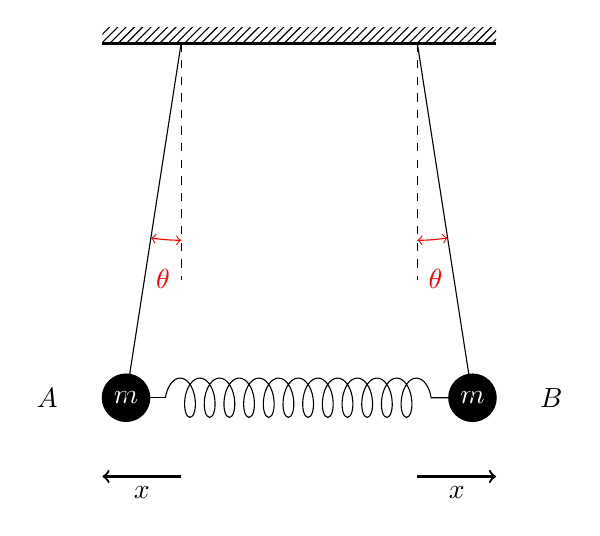
\begin{tikzpicture}
\coordinate (a) at ($(0,0)+(-0.7,0.5)$);
\coordinate (b) at ($(3,0)+(0.7,0.5)$);
\coordinate (pivot1) at (0,5);
\coordinate (pivot2) at (3,5);
\node[circle,fill=black,inner sep=1mm] at (a) {$\textcolor{white}{m}$};
\node[circle,fill=black,inner sep=1mm] at (b) {$\textcolor{white}{m}$};
\node at ($(a)+(-1,0)$) {$A$};
\node at ($(b)+(1,0)$) {$B$};
\draw ($(a)+(0.2,0)$) -- +(0.3,0);
\draw[decoration={aspect=0.5, segment length=2.5mm, amplitude=2.5mm,coil},decorate] ($(a)+(0.5,0)$) -- ($(b)+(-0.3,0)$); 
\draw (pivot1) -- (a); 
\draw (pivot2) -- (b); 
\draw[dashed] (0,5) -- ++(0,-3) node (end1){};
\draw[dashed] (3,5) -- ++(0,-3) node (end2){};
\draw [->, thick] ($(0,5)+(0,-5.5)$) -- ++(-1,0);
\node[anchor=north] at ($(0,5)+(-0.5,-5.5)$) {$x$};
\draw [->, thick] ($(3,5)+(0,-5.5)$) -- ++(1,0);
\node[anchor=north] at ($(3,5)+(0.5,-5.5)$) {$x$};
\draw pic["$\textcolor{red}{\theta}$",draw=red,<->,angle eccentricity=1.2, angle radius=2.5cm] {angle=a--pivot1--end1};
\draw pic["$\textcolor{red}{\theta}$",draw=red,<->,angle eccentricity=1.2, angle radius=2.5cm] {angle=end2--pivot2--b};
\fill [pattern = north east lines] (-1,5) rectangle (4,5.2);
\draw[thick] (-1,5) -- (4,5);
\end{tikzpicture}

\end{subfigure}
\caption{The two normal modes}
\label{fig:cp_two_normal}
\end{figure}

\section{Superposition of the normal modes}

Let us now try to solve equations \ref{equation:two_cp_pendulums_1} and \ref{equation:two_cp_pendulums_2} for general initial conditions. The 
symmetry of the two equations suggests that adding and subtracting them might give some joy:

\begin{align*}
\ddot{x_a} + \ddot{x_b} + \omega_0^2(x_a + x_b) &= 0\\
\ddot{x_a} - \ddot{x_b} + (\omega_0^2 + 2\omega_c^2)(x_a - x_b) &= 0
\end{align*}

Indeed, these are two simple harmonic motions. Introducing the \textit{normal co-ordinates} $q_1 = x_a + x_b$ and $q_2 = x_a - x_b$,

\begin{align*}
\ddot{q_1} + \omega_0^2q_1 &= 0\\
\ddot{q_2} + \omega\prime^{2}q_2 &= 0
\end{align*}

whose solutions are

\begin{align*}
q_1 = C\cos{\omega_0t}\\
q_2 = D\cos{\omega\prime t}
\end{align*}

where we have already assumed two initial conditions (initial phases are zero) for simplicity. In terms of our original co-ordinates,

\begin{align*}
x_a = \frac{1}{2}(q_1 + q_2) &= \frac{1}{2}C\cos{\omega_0t} + \frac{1}{2}D\cos{\omega\prime t}\\
x_b = \frac{1}{2}(q_1 - q_2) &= \frac{1}{2}C\cos{\omega_0t} - \frac{1}{2}D\cos{\omega\prime t}
\end{align*}

We see that the general motion of the oscillator is a superposition of it's normal modes. This is a general result for any number of coupled oscillators. Let us now consider what happens when we pull aside pendulum $A$ by a small amount while keeping $B$ fixed, ie. the above equations
subject to the initial conditions at $t=0$

\begin{align*}
x_a &= A_0\\
\dot{x_a} &= 0\\
x_b &= 0\\
\dot{x_b} &= 0\\
\end{align*}

We obtain

\begin{align*}
x_a &= A_0\cos{\frac{\omega\prime - \omega_0}{2}t}\cos{\frac{\omega\prime + \omega_0}{2}t}\\
x_b &= A_0\sin{\frac{\omega\prime - \omega_0}{2}t}\sin{\frac{\omega\prime + \omega_0}{2}t}\\
\end{align*}

These motions are plotted in figure . We see that $A$ starts swinging initially, but it's amplitude continuously decreases. Pendulum $B$, initially
at rest, starts oscillating and soon the amplitudes of $A$ and $B$ become equal. The amplitude of $A$ then diminishes towards zero and the amplitude
of $B$ becomes that of $A$ originally. The spring is therefore acting as a kind of energy transfer agent between the two pendulums.



\end{document}
